% Hero pipeline diagram for the project README.
% Build:  ./build.sh   (pdflatex -> pdf2svg)
%
% Deliberately self-contained: no \includegraphics, so it compiles from any
% directory with a plain TeX Live install.

\documentclass[border=12pt]{standalone}

\usepackage{tikz}
\usepackage{amssymb}                  % \blacksquare, used by the legend
\usetikzlibrary{positioning, arrows.meta, calc, fit, backgrounds}

\definecolor{cC}{HTML}{2A78D6}        % C components
\definecolor{cCbg}{HTML}{E4EEFB}
\definecolor{cPy}{HTML}{1BAF7A}       % Python components
\definecolor{cPybg}{HTML}{E1F5EE}
\definecolor{cDb}{HTML}{EB6834}       % storage / SQL
\definecolor{cDbbg}{HTML}{FCEBE3}
\definecolor{cData}{HTML}{898781}     % external data
\definecolor{cDatabg}{HTML}{F0EFEC}
\definecolor{ink}{HTML}{0B0B0B}
\definecolor{ink2}{HTML}{52514E}

\begin{document}
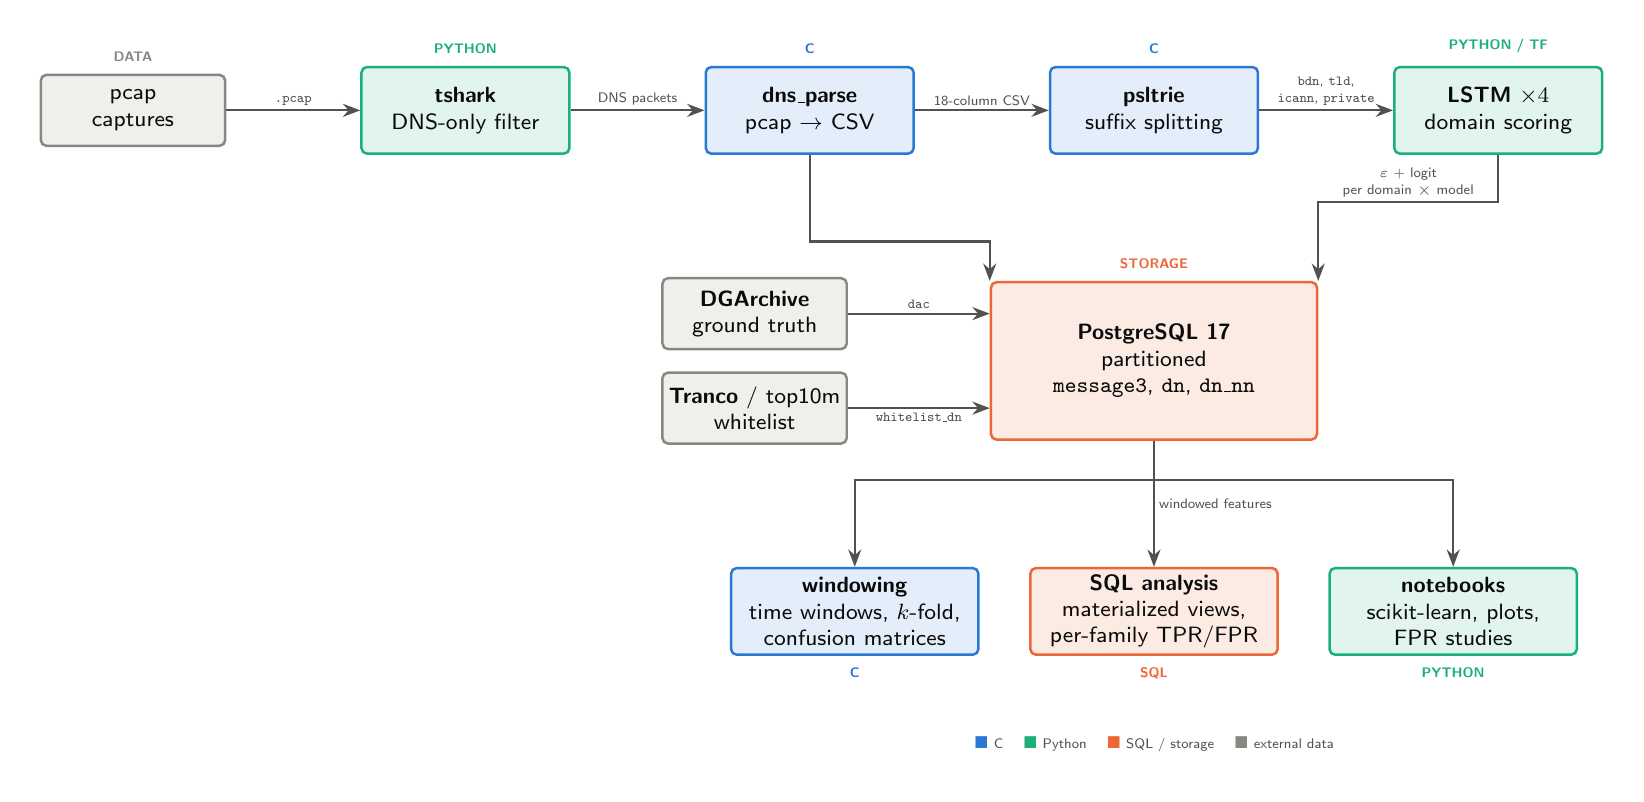
\begin{tikzpicture}[
    background rectangle/.style={fill=white},
    show background rectangle,
    font=\sffamily,
    node distance=8mm,
    box/.style={
        rectangle, rounded corners=2pt, draw=#1, line width=0.9pt,
        minimum height=11mm, text width=25mm, align=center,
        inner sep=2pt, text=ink, font=\sffamily\footnotesize
    },
    cbox/.style={box=cC,   fill=cCbg},
    pybox/.style={box=cPy, fill=cPybg},
    dbbox/.style={box=cDb, fill=cDbbg},
    databox/.style={box=cData, fill=cDatabg, minimum height=9mm, text width=22mm},
    arr/.style={-{Stealth[length=2.2mm]}, draw=ink2, line width=0.8pt},
    lbl/.style={font=\sffamily\tiny, text=ink2, inner sep=1.5pt, midway, align=center},
    tag/.style={font=\sffamily\tiny\bfseries, text=#1, inner sep=0pt},
]

% ---------------------------------------------------------------- ingest row
\node (pcap)   [databox]                        {pcap\\captures};
\node (tshark) [pybox, right=17mm of pcap]      {\textbf{tshark}\\DNS-only filter};
\node (parse)  [cbox,  right=17mm of tshark]    {\textbf{dns\_parse}\\pcap $\rightarrow$ CSV};
\node (psl)    [cbox,  right=17mm of parse]     {\textbf{psltrie}\\suffix splitting};
\node (lstm)   [pybox, right=17mm of psl]       {\textbf{LSTM} $\times 4$\\domain scoring};

\node[tag=cData, above=1.5mm of pcap]   {DATA};
\node[tag=cPy,   above=1.5mm of tshark] {PYTHON};
\node[tag=cC,    above=1.5mm of parse]  {C};
\node[tag=cC,    above=1.5mm of psl]    {C};
\node[tag=cPy,   above=1.5mm of lstm]   {PYTHON / TF};

\draw [arr] (pcap)   -- node[lbl, above] {\texttt{.pcap}}      (tshark);
\draw [arr] (tshark) -- node[lbl, above] {DNS packets}         (parse);
\draw [arr] (parse)  -- node[lbl, above] {18-column CSV}       (psl);
\draw [arr] (psl)    -- node[lbl, above] {\texttt{bdn}, \texttt{tld},\\\texttt{icann}, \texttt{private}} (lstm);

% ---------------------------------------------------------------- database
\node (db) [dbbox, below=16mm of psl, text width=40mm, minimum height=20mm]
    {\textbf{PostgreSQL 17}\\\footnotesize partitioned \texttt{message3}, \texttt{dn}, \texttt{dn\_nn}};
\node[tag=cDb, above=1.5mm of db] {STORAGE};

\draw [arr] (lstm.south) -- ++(0,-6mm) -| node[lbl, above, pos=0.25]
    {$\varepsilon$ + logit\\per domain $\times$ model} (db.north east);
\draw [arr] (parse.south) -- ++(0,-11mm) -| (db.north west);

% ------------------------------------------------------- ground truth inputs
\node (dac) [databox, left=18mm of db, yshift=6mm]  {\textbf{DGArchive}\\ground truth};
\node (wl)  [databox, left=18mm of db, yshift=-6mm] {\textbf{Tranco} / top10m\\whitelist};

\draw [arr] (dac) -- node[lbl, above] {\texttt{dac}}          (dac -| db.west);
\draw [arr] (wl)  -- node[lbl, below] {\texttt{whitelist\_dn}} (wl  -| db.west);

% ---------------------------------------------------------------- analysis row
\node (win)  [cbox,  below=16mm of db, xshift=-38mm, text width=30mm]
    {\textbf{windowing}\\time windows, $k$-fold,\\confusion matrices};
\node (sql)  [dbbox, below=16mm of db, text width=30mm]
    {\textbf{SQL analysis}\\materialized views,\\per-family TPR/FPR};
\node (nb)   [pybox, below=16mm of db, xshift=38mm, text width=30mm]
    {\textbf{notebooks}\\scikit-learn, plots,\\FPR studies};

\node[tag=cC,  below=1.5mm of win] {C};
\node[tag=cDb, below=1.5mm of sql] {SQL};
\node[tag=cPy, below=1.5mm of nb]  {PYTHON};

\draw [arr] (db.south) -- ++(0,-5mm) -| (win.north);
\draw [arr] (db.south) -- node[lbl, right] {windowed features} (sql.north);
\draw [arr] (db.south) -- ++(0,-5mm) -| (nb.north);

% ---------------------------------------------------------------- legend
\node (leg) at ($(sql.south) + (0,-9mm)$) [anchor=north, font=\sffamily\tiny, text=ink2]
    {\begin{tabular}{@{}l@{}}
        \textcolor{cC}{$\blacksquare$}~C \quad
        \textcolor{cPy}{$\blacksquare$}~Python \quad
        \textcolor{cDb}{$\blacksquare$}~SQL / storage \quad
        \textcolor{cData}{$\blacksquare$}~external data
     \end{tabular}};

\end{tikzpicture}
\end{document}
